%%=============================================================================
%% Methodologie
%%=============================================================================

\chapter{\IfLanguageName{dutch}{Methodologie}{Methodology}}
\label{ch:methodologie}
In het vorige hoofdstuk werd een overzicht gegeven van maatregelen die het mogelijk maken voor een organisatie om beter te voldoen aan de GDPR. Voor enkele van die maatregelen is een verdere uitwerking vereist. Deze uitwerking volgt in dit hoofdstuk.  
De twee verder uitgewerkte maatregelen zijn data-retentie, en het uitgelichte deel over het extraheren van persoonlijke data uit foto's en tekst (=niet-structurele informatie). 

Opmerking: in dit hoofdstuk worden technische begrippen gebruikt. Voor een uitleg van deze begrippen, die hoofdstuk 2: stand van zaken. 

%\subsection{Data Protection}

%% TODO: Hoe ben je te werk gegaan? Verdeel je onderzoek in grote fasen, en
%% licht in elke fase toe welke stappen je gevolgd hebt. Verantwoord waarom je
%% op deze manier te werk gegaan bent. Je moet kunnen aantonen dat je de best
%% mogelijke manier toegepast hebt om een antwoord te vinden op de
%% onderzoeksvraag.
\section{Data retention}

Zoals beschreven in het hoofdstuk Maatregelen (3.6) is het belangrijk als organisatie een juiste beslissingen te maken over hoe lang persoonlijke data zal worden bijgehouden. 

InSites Consulting ontvangt elke dag een zekere hoeveelheid aan data, waarvan slechts een deel als persoonlijke data kan worden aanzien. Oorspronkelijk, voor de GDPR, werd alle data voor onbepaalde tijd bijgehouden. 

Een eerste stap die hier moet ondernomen worden is de persoonlijke data scheiden van andere data. Op deze manier kunnen ze verder gaan met het bijhouden van alle data die buiten de GDPR valt in welke mate ze zelf willen, en de data die wel persoonlijke informatie bevat binnen een bepaalde tijdspanne gaan verwijderen. 

Hoe is dit aangepakt? Eerst is het probleem gegeneraliseerd: het is niet nodig bij elke ingevulde vragenlijst elke vraag afzonderlijk te gaan beoordelen. 
Dit zou enkel tot nodeloos ingewikkelde implementaties leiden, met minimaal voordeligere resultaten. 

Daarom is het beslissingsniveau of data al dan niet persoonlijke info kan bevatten, op 'Activity'-niveau gelegd (een activity bij InSites Consulting is een kwantitatief of kwalitatief onderzoek, zoals een vragenlijst). Bij creatie van een Activity kan worden beslist of deze over persoonlijke onderwerpen zal gaan, en/of er een mogelijkheid zal zijn dat er data wordt ontvangen van participanten met persoonlijke informatie. Deze beslissing wordt gemaakt door een een werknemer van InSites consulting, die als Administrator op de 'Square'-omgeving activities kan aanmaken. 
Dit is op een eenvoudig wijze opgelost door middel van een 'checkbox' op de pagina waar de Activity wordt aangemaakt. (Zie figuur) 

\begin{figure}[h]
	\centering
	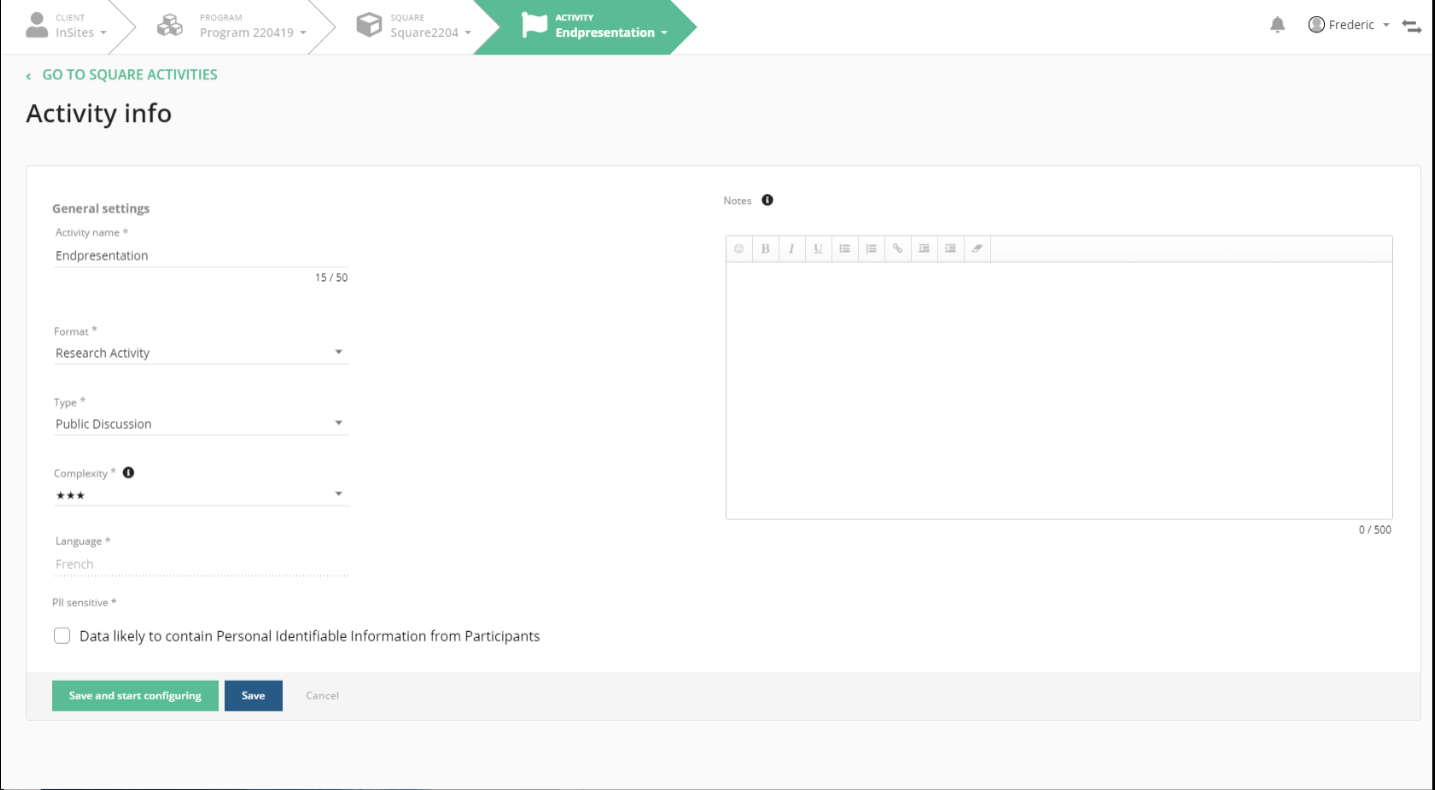
\includegraphics[width=\linewidth, scale=0.5]{screenshot_create_activity}
	\label{fig:create_activity}
	\caption{Ingebouwde beveiligingsopties excel-worksheets.}
\end{figure}


Op deze manier kan in de databasetabel met info over de Activities een extra kolom worden toegevoegd: PII-sensitive; met een bit-waarde (0 bij niet persoonlijke info, 1 voor wel persoonlijke info). 
Dan kan, bij het bereiken van een bepaalde datum na creatie van deze Activity, afhankelijk van de waarde binnen de PII-sensitive-tabel, een activity verwijderd worden. Hierbij worden alle gegevens, gehaald uit die Activity, mee verwijderd of geanonimiseerd. Dankzij deze oplossing (=de checkbox) kan dit geautomatiseerd gebeuren, en is er geen nood aan een werknemer die alles handmatig overloopt. 

Een manier om dit geautomatiseerd te doen is via een \textbf{stored procedure}. Een stored procedure is een programma dat bewaard wordt binnen de database. Een mogelijkheid is bijvoorbeeld om een stored procedure op te stellen die elke dag op een bepaald uur controleert hoelang de aanmaakdata van alle Activities verstreken zijn. De DPO kan een beslissing maken hoelang persoonlijke data mag bijgehouden worden, en van zodra een Activity zijn maximum termijn heeft bereikt, worden de gegevens verwijderd. Op deze manier zorg je ervoor dat je data die eventueel persoonlijke informatie kan bevatten, niet onnodig lang bijhoudt, zoals voorgeschreven in de GDPR.  

\subsection{Data Access Control}
De data die Insites consulting ontvangt via het uitgevoerde marktonderzoek moet worden beschermd. Hier kunnen nog op enkele plaatsen verbeteringen aangebracht worden: 

Bijvoorbeeld, op verschillende plaatsten binnnen de software van InSites Consulting is het voor admin users (=werknemers die marktonderzoek uitvoeren) mogelijk om exports te nemen van data. Een export is een lijst van gegevensdie in de vorm van een Excel-bestand lokaal opgeslagen bij werknemer.
Vaak bevat zo'n export persoonlijke data. Tenzij de data op de juiste manier beschermd is, en up-to-date wordt gehouden (wat niet het geval is bij InSites), voldoet dit niet aan de voorwaarden van de GDPR. 

\begin{figure}[h]
	\centering
	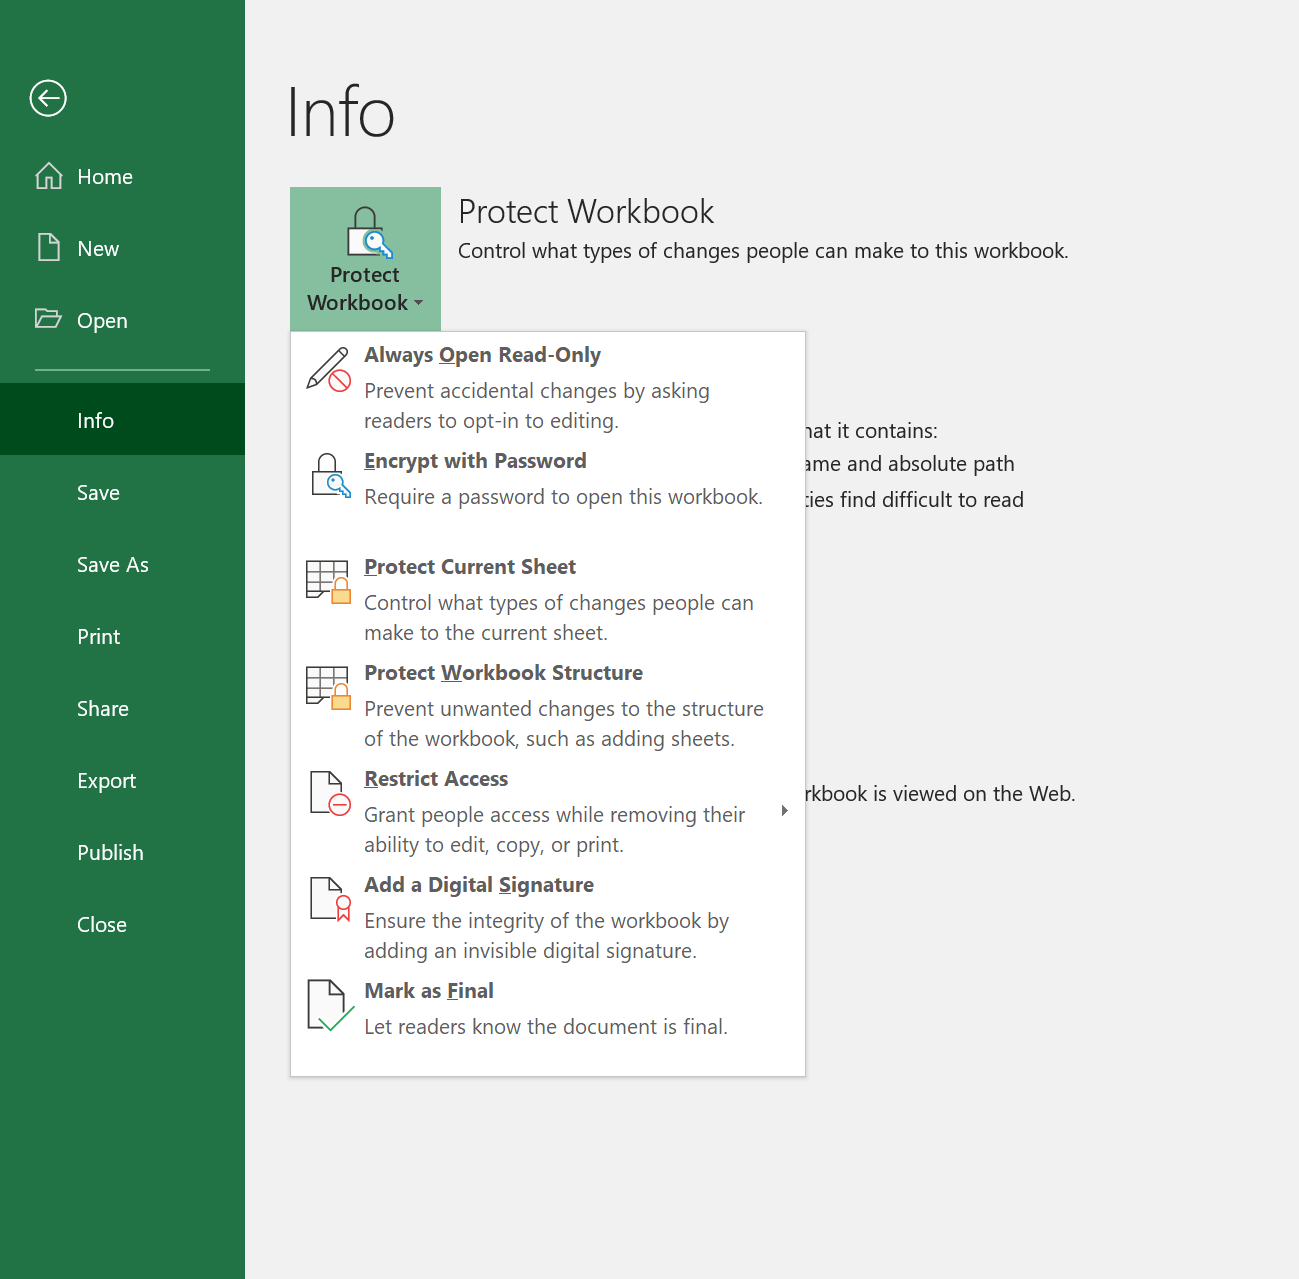
\includegraphics[width=\linewidth, scale=0.5]{Excel_beveiliging_opties}
	\label{fig:excelbeveiliging}
	\caption{Ingebouwde beveiligingsopties excel-worksheets.}
\end{figure}


Excel biedt zelf enkel \textbf{oplossingen} aan \textbf{om data te beschermen} (zie figuur 4.2). Eén van de opties is om een Excel-bestand te beschermen met een \textbf{wachtwoord}. Dat lijkt misschien overbodig, aangezien enkel users met administrator rechten (wat wachtwoord-beveiligd is) binnen InSites een export kunnen nemen, maar het biedt wel degelijk extra voordelen. Als je een wachtwoord instelt, blijft dit ook van kracht eens het Excel-bestand gedownload is en lokaal (op de pc van een werknemer) opgeslagen staat. Zo heb je meer veiligheid in geval van een datalek waarbij data van pc's vrijgegeven is. Of wanneer iemand zijn wachtwoord is gelekt (bijvoorbeeld via phishing\footnote{Volgens www.phishing.org is phising een cybermisdaad waarbij een doelwit via email, telefoon of sms gecontacteerd wordt, door iemand die zich valselijk voordoet als een legitieme instantie, met als bedoeling ongewild persoonlijke informatie, bankgegevens, enzoverder te bemachtigen.}) om op de InSites-omgeving te graken. In dat geval zou de binnendringer wel de excel-sheet kunnen downloaden, maar de inhoud niet lezen. \\

Een aanvullende ingebouwd optie, \textbf{'Restrict Access'}, biedt de mogelijkheid om gebruikers bepaalde rechten (zoals data kopiëren, doormailen, enzoverder) te ontnemen. Door deze instellingen aan te passen kan vermeden worden dat de data aanwezig in de export ongewild verder verspreid wordt. 

Wat reeds gebeurd bij InSites is het loggen in een database wie wanneer een export heeft genomen. Dit is reeds een goede maatregel in verband met data retentie. Wat hier nog extra zou kunnen gedaan worden is, op het moment de export genomen wordt, de InSites werknemer te vragen (via een popup of email) om de data niet langer bij te houden dan nodig. Bijgevolg kunnen op regelmatige tijdstippen controles uitgevoerd worden aan de hand van de data in de logging, of de werknemer in kwestie effectief de data heeft verwijderd. 

\section{Aanvraag tot verwijderen persoonlijke data}

In het eerste deel van dit hoofdstuk werd ingegaan op het verwijderen van data na een lange periode. Maar wanneer een gebruiker een verzoek indient om zijn persoonlijke data te verwijderen, voor het eind van deze periode, moet op een andere manier aan de slag gegaan worden. Het is geen optie om volledige Activities te verwijderen op dit moment, omdat die nog actief kunnen zijn, de data nog van belang kan zijn, enzoverder. Er moet een poging gedaan worden enkel de gevraagde persoonlijke info te vinden en te verwijderen. 
 
\subsection{Mogelijkheid}
In de eerste plaats moet er een mogelijkheid zijn om deze aanvraag in de dienen. De manier waarop maakt weinig uit. Het kan door een knop op het platform/website/... ter beschikking te stellen als "Verwijder al mijn gegevens", waarna alles geautomatiseerd verwerkt wordt. Het kan ook door in je privacy policy mee te delen dat een mail kan gestuurd worden met deze aanvraag. De mogelijkheden zijn eindeloos. 
 
\subsection{Insites Consulting en niet-gestructureerde data}

In het geval van InSites Consulting (en dit kan dus ook voor andere organisaties gelden), bevat de verwerkte data meer dan enkel structurele data. \\
Voor het marktonderzoek dat bij InSites wordt uitgevoerd op de 'Square', worden vaak openbare discussies opgesteld over producten. Hierbij kunnen gebruikers van de Square openbaar reageren in open velden. Bijgevolg beschikt InSites over veel niet-gestructureerde data. 
 De uitdaging is om hierin geautomatiseerd als persoonlijke info te herkennen, zodat het kan verwijderd worden indien nodig.
 
In de volgende secties worden geautomatiseerde oplossingen te voorzien voor dit probleem. 
In stand van zaken werden hiervoor twee aanbieders uitgelicht, namelijk Microsoft Azure en Google cloud. In kader van de samenwerking met InSites Consulting is gekozen om de volgende applicaties uit te werken met Azure, aangezien InSites daar reeds klant is.

\subsection{ConsoleApplicatie PII uit text.}
In dit deel wordt een applicatie aangeboden voor het geautomatiseerd zoeken naar persoonlijke gegevens in tekst. 

Een goed startpunt om een applicatie op te zetten die gebruik maakt van Azure Cognitive Services is hun documentatie. \textcite{Services2019} \\
Hier wordt uitgelegd hoe je aan de slag kan om een applicatie te bouwen die communiceert met de cognitive services-API. De bedoeling is om geautomatiseerd stukken niet-gestructureerde tekst te evalueren, en deze te controleren op aanwezigheid van  persoonlijke informatie. Zodat, indien hiertoe een aanvraag komt, deze data kan verwijderd worden. 

\subsubsection{Stap 1: ConsoleApp die tekst inleest}
Cognitive services biedt voor textanalyse een SDK aan.
 Deze SDK geeft toegang tot de verschillende cognitive services language API's, die zijn in staat tekst te analyseren en info uit te extraheren. In dit project is gekozen om te code te schrijven in de programmeertaal C\# omdat dit te voorkeur is van InSites Consulting. Microsoft biedt de SDK ook nog aan voor Python en Ruby. Als een onderneming geen gebruik wil maken van de aangeboden SDK, maar rechtstreeks API-calls wil uitvoeren, kan dit met GO, Java, Node.JS, PHP, Python of Ruby.\\

\begin{figure}[h]
	\centering
	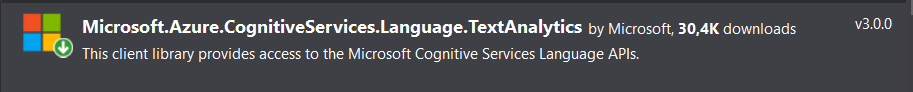
\includegraphics[width=\linewidth]{Ms_Cognitive_Services_TextAnalyticsSDK}
	\label{fig:textanalyticsSDK}
	\caption{SDK library van Microsoft die API's bevat voor tekstanalyse.}
\end{figure}

Wat de textanalyse-service aanbiedt is het herkennen van entiteiten in zinnen. In tabel 4.1 staat een overzicht van welke entiteiten worden ondersteund en kunnen worden herkend. \textcite{Hill2019}
In de eerste kolom vindt je het type entiteiten, tweede kolom een voorbeeld, en in de derde kolom of deze entiteiten voor dit onderzoek interessant zijn: of ze mogelijks persoonlijke informatie bevatten. 

\begin{table}

	\begin{tabularx}{\linewidth}{ |X|l|l| } 
        	
	\hline
	Entiteit - Type & Voorbeeld & Mogelijk PII \\ [0.5ex]
	
	\hline\hline
	Persoon & Jeff & \checkmark \\ \hline 
	Locatie & 'Parijs', 'Redmond, Washington & \checkmark \\ \hline  
	Organisatie & Microsoft & \checkmark \\ \hline 
	Kwantiteit:Percentage, dimensie, temperatuur,... & 50\%, 10miles, ... & \\ \hline 
	Kwantiteit:Leeftijd & 30 years old & \checkmark \\ \hline 
	URL & www.bing.com & \checkmark \\ \hline 
	Email & test@test.com & \checkmark \\ \hline 
	Datum/tijd & 2nd may 2017 & \\ \hline 
	
	\hline

\end{tabularx}
\caption{Ingebouwde beveiligingsopties excel-worksheets.} 
\end{table}
De eerste stap is om een .NET-core project aan te maken (Console-app), en de Cognitive Services SDK te installeren.  
Daarna om van uit dit project  de API's van cognitive services aanspreken. In de eerste testfase werken we met mockdata (= mockdata is geen echte data maar verzonnen data met als doel te voldoen aan de benodigde data voor het onderzoek). Je ziet in onderstaand codevoorbeeld enkele zinnen tekst. De bedoeling is deze zinnen te ontleden in entiteiten, en dan de gevonden entiteiten verder te beoordelen. 
Hiervoor wordt de data geanalyseerd door de EntitiesAsync-methode die ingebouwd is in de SDK. In listing 4.1 zijn de net omschreven stappen uitgewerkt in C\#, op lijn 9 gebeurt de effectieve communicatie met de API. 

\begin{lstlisting}[frame=single, caption={Een deel van de console-applicatie die de cognitive services API aanspreekt om text te ontleden in entiteiten}, captionpos=b]
var inputDocuments = new MultiLanguageBatchInput(
new List<MultiLanguageInput>
{
	new MultiLanguageInput("en", "1", "Microsoft was founded by Bill Gates and Paul Allen on April 4, 1975, to develop and sell BASIC interpreters for the Altair 8800."),
	new MultiLanguageInput("en", "3", "My emailadress is frederic.Terryn@hotmail.com"), 
	new MultiLanguageInput("en", "4", "Hi, @loredana16, do you like my picture?")
});
//...
var entitiesResult = await client.EntitiesAsync(false, inputDocuments);

// Printing recognized entities
foreach (var document in entitiesResult.Documents)
{
	Console.WriteLine($"Document ID: {document.Id} ");
	
	Console.WriteLine("\t Entities:");
	foreach (var entity in document.Entities)
	{
		Console.WriteLine($"\t\tName: {entity.Name},\tType: {entity.Type ?? "N/A"},\tSub-Type: {entity.SubType ?? "N/A"}");
		foreach (var match in entity.Matches)
		{
			Console.WriteLine($"\t\t\tOffset: {match.Offset},\tLength: {match.Length},\tScore: {match.EntityTypeScore:F3}");
		}
	}
}
\end{lstlisting}

\subsubsection{Stap 2: Entiteiten wegfilteren}

Na het uitvoeren van bovenstaande methode, geeft de API een document terug met de herkende entiteiten. (Zie listing 4.2)
\begin{lstlisting}[frame=single, caption={Resultaten in de vorm van entiteiten uit de textanalyse}, captionpos=b]
Document ID: 1
Entities:
Name: Microsoft,        Type: Organization,     Sub-Type: N/A
Offset: 0,      Length: 9,      Score: 1,000
Name: Bill Gates,       Type: Person,   Sub-Type: N/A
Offset: 25,     Length: 10,     Score: 1,000
Name: Paul Allen,       Type: Person,   Sub-Type: N/A
Offset: 40,     Length: 10,     Score: 0,999
Name: April 4,  Type: Other,    Sub-Type: N/A
Offset: 54,     Length: 7,      Score: 0,800
Name: April 4, 1975,    Type: DateTime, Sub-Type: Date
Offset: 54,     Length: 13,     Score: 0,800
Name: BASIC,    Type: Other,    Sub-Type: N/A
Offset: 89,     Length: 5,      Score: 0,800
Name: Altair 8800,      Type: Other,    Sub-Type: N/A
Offset: 116,    Length: 11,     Score: 0,800
Document ID: 3
Entities:
Name: frederic.Terryn@hotmail.com,      Type: Email,    Sub-Type: N/A
Offset: 18,     Length: 27,     Score: 0,800
Document ID: 4
Entities:
\end{lstlisting}

De bedoeling is nu, om bepaalde delen van zinnen weg te laten, afhankelijk van welk type entiteit ze zijn. 
Bijvoorbeeld: als een persoon (naam) herkend wordt, kan deze naam uit de zin weggefilterd worden, omdat een naam persoonlijke informatie is. 
Er wordt gefilterd op alle entiteit waar in tabel 4.1 in de derde kolom een vinkje staat. 

De API van Microsoft geeft enkel terug welke entiteiten er zijn herkend, er is geen ingebouwde functionaliteit voor het filteren. Dit kan door zelf enkele methodes te schrijven. In de methodes in listing 4.2 zullen de herkende entiteiten overlopen worden, en indien ze van een type zijn die persoonlijke informatie bevatten, vervangen worden door 'XXX'. 
\begin{lstlisting}[frame=single, caption={Gevonden, persoonlijke informatie bevattende, entiteiten filteren}, captionpos=b]
                foreach (var entity in document.Entities)
{
if (entity.Type == "Person" || entity.Type == "Email" || entity.Type == "Location" || entity.Type == "DateTime")
{

if (currenctsentence.Value != null)
{
anonymoussentence = ReplaceFirstOccurrence(anonymoussentence, entity.Name, "XXX");
} 

}

       private static string ReplaceFirstOccurrence(string Source, string Find, string Replace)
{
int Place = Source.IndexOf(Find);
if (Place >= 0)
{
string result = Source.Remove(Place, Find.Length).Insert(Place, Replace);
return result;
}
else return Source;
}
\end{lstlisting}

Als mockdata worden 20 zinnen genomen. In deze 20 zinnen zit op allerlei verschillende manieren persoonlijke informatie. Het resultaat zie je in tabel 4.2.

\begin{table}
	\begin{tabularx}{\linewidth}{ |X|X| } 
	\hline
	Originele zin & Gefilterde zin \\ \hline \hline
	Microsoft was founded by Bill Gates and Paul Allen on April 4, 1975, to develop and sell BASIC interpreters for the Altair 8800. & Microsoft was founded by XXX and XXX on XXX, to develop and sell BASIC interpreters for the Altair 8800.\\
	this is a test & this is a test\\
	My emailadress is frederic.Terryn@hotmail.com &  My emailadress is XXX \\
	I think you can call him on +32472123456 & I think you can call him on +32472123456 \\
	I was born and December I live in Sint-Jacobsstraat 16 &  I was born and December I live in XXX-Jacobsstraat 16 \\
	Hi, @loredana16, can you like my picture? & Hi, @loredana16, can you like my picture? \\
	Yes, that's a good answer &  Yes, that's a good answer \\
	3, Baker Street, London & 3, XXX, XXX \\
	My mother thinks I suffer from HIV & My mother thinks I suffer from HIV \\
	My income is 2150 a year & My income is 2150 XXX \\
	This table is round &  This table is round \\
	I had a call from +34 456 487 654 &  I had a call from +34 456 487 654 \\
	I don't want to work anymore, I'm done, i hate it! &  I don't want to work anymore, I'm done, i hate it! \\
	My name is Lewis and i just won EuroMillions &  My name is XXX and i just won Euromillions. \\
	Yes i totally agree with all what you say. &  Yes i totally agree with all what you say. \\
	No, i've had enough. I said, enough! &  No, i've had enough. I said, enough! \\
	My kids names are Lewis, lolita and Franklin &  My kids names are XXX, lolita and XXX \\
	These are 3 names: Louis, Charlotte en Carl&  These are 3 names: Louis, XXX en XXX \\
	The world is round & The world is round \\
	\hline
	
	\end{tabularx}
\caption{In deze tabel wordt in de eerste kolom de te filteren mockdata getoond. In de rechtse kolom zie je het resultaat na het filteren.}
\end{table}

\subsubsection{Stap 3:Analyseren resultaten}

In de 2de kolom van tabel 4.2 staat de gefilterde data. Het is duidelijk dat op bepaalde plaatsen persoonlijke data is verwijderd. Zoals in de eerste zin, zijn de namen, en ook het jaartal, weggefilterd. Ook de zin 'My emaildress is frederic.terryn@hotmail.com' lijkt gefilterd zoals gewenst: het emailadres kan al persoonlijke informatie gezien worden en is dus geanonimiseerd naar 'My emailadress is XXX'. 

Er zijn echter \textbf{heel wat plaatsen waar de persoonlijke informatie niet gefilterd is}. 
In de zinnen 'My kids are Lewis, lolita and Franklin', en 'These are 3 names: Louis, Charlotte en Carl' blijft telkens één naam ongefilterd. 
Ook telefoonnummers aanwezig in de zinnen zijn nog aanwezig. In de zin 'I was born and December I live in Sint-Jacobsstraat', is enkel het eerste deel van de straatnaam gefilterd.

De redenen waarom de filter niet perfect werkt, zijn gebaseerd op vermoedens aangezien Microsoft de precieze werking van de API niet deelt. Een reden kan zijn dat \textbf{de API enkel Engelstalige info verwerkt.} \\ Voor InSites Consulting is dit al een probleem, aangezien er gebruikers zijn van over de hele wereld, en niet enkel Engelstalige informatie moet worden gefilterd. 
Dit kan verklaren waarom 'Sint-Jacobsstraat' niet herkend werd, aangezien het Nederlandstalig is, en 'Baker Street' wel. 
Het woord 'Sint' uit 'Sint-Jacobsstraat' is wel degelijk herkend als een locatie (zie figuur 4.4), maar het vervolg van het woord niet meer. 
 
\begin{figure}[h]
    \includegraphics[width=\linewidth]{sintPNG.png}
    \caption{Cognitive services - Face recognition. Links de foto, rechts een JSON-file met herkende elementen.}
    \label{fig:sint}
\end{figure}

Als bijkomende test (zie figuur 4.5), worden nog enkele straatnamen en vlaamse persoonsnamen gecontroleerd.
Als resultaat worden 9 van de 10 namen en straatnamen gefilerd. De test lijkt goed gelukt. Al is er echter te zien op foto (b) dat de straatnamen herkend zijn als persoonsnamen. Hier kan de vraag gesteld worden of de API betrouwbaar is. Er kan niet van uitgegaan worden dat in de toekomst elke straatnaam als persoon zal worden herkend. 

\begin{figure}[h]
    \centering
    \begin{subfigure}{0.45\textwidth}
        \centering
        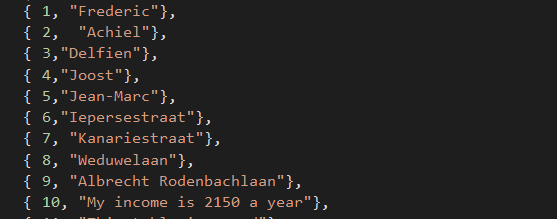
\includegraphics[width=.7\linewidth]{NamesandStreets.png}
        \caption{10 niet Engelstalige persoons- en straatnamen}
        \label{fig:namesandstreets}
    \end{subfigure}%
    \begin{subfigure}{0.45\textwidth}
        \centering
        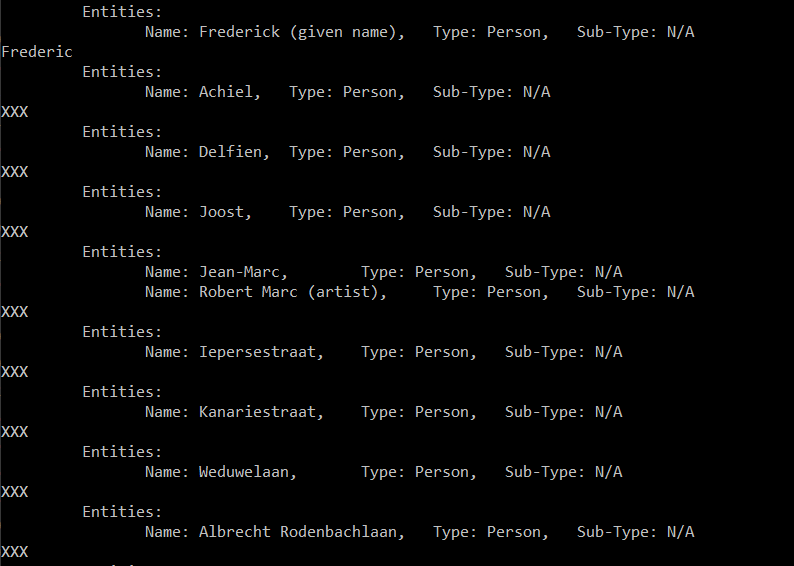
\includegraphics[width=.7\linewidth]{names.PNG}
        \caption{Het resultaat van de applicatie, als de data van foto a wordt ingevoerd.}
        \label{fig:names}
    \end{subfigure}
    \caption{Een extra test of de cognitive services niet-Engelstalige persoonnamen en straatnamen herkent.}
    \label{fig:extratest}
\end{figure}

Daarnaast moet er nog rekening mee gehouden worden dat veel soorten persoonlijke data, zoals ziektebeelden en telefoonnummers (in de Europese vorm) in de tabel 4.1, nog niet herkend worden als type-entiteit en ook hier niet kan op gefilterd worden. 

\subsubsection{Stap 4: optimalisatie}
	
Voorlopig kan de API dus gedeeltelijk persoonlijke data filteren uit niet-gestructureerde, maar er kan niet van uitgegaan worden dat alle persoonlijke informatie zal herkend worden. \textbf{Het blijft dus voorlopig een hulpmiddel dat extra's kan aanbieden, maar geen eindoplossing}. 

Voor InSites (en andere ondernemingen in het algemeen) kan het wel interessant zijn om zelf aanvullingen te maken op wat de Artifiële Intelligentie binnen de textanalyse-API herkent. \\

Bijvoorbeeld: op de Square kunnen verschillende participanten elkaar taggen. Dit is altijd onder de vorm '@gebruikersnaam'. Dit is dus structurele data, die aanwezig is binnenin niet-structurele data. De herkenning hiervan kan door middel van reguliere expressies\footnote{Een reguliere expressie is een manier om patronen te beschrijven waarmee een computer tekst kan herkennen} tot de voegen aan de C\# applicatie.
De reguliere expressie '@[A-z,1-9]+' komt overeen met een '@'-teken gevolgd door letters en/of cijfers, tot de eerste spatie. Als je hierop filtert in de consoleapplicatie krijg je volgende resultaten (tabel 4.3).

  \begin{table}
      
      \begin{tabularx}{\linewidth}{ |X|l| } 
          
          \hline
          Mockdata ongefilterd & Mockdata gefilterd \\

          \hline\hline
          Hi, @loredana16, do you like my picture?  & Hi, XXX, do you like my picture? \\
          I agree with @lewis! & I agree with XXX \\
          What you say! @anonymoususer328! & What you say! XXX! \\
          Nope, i don't agree @moderator & Nope, i don't agree XXX \\
          @User345, what did you mean? &   XXX, what did you mean?\\
          \hline
          
      \end{tabularx}
      \caption{Mockdata gefilterd met reguliere expressies.} 
  \end{table}



\subsection{ConsoleApplicatie PII uit foto's.}
Naast tekst biedt Azure ook services aan om foto's te analyseren. Niet-structurele data kan ook voorkomen in de vorm van foto's. Bij een aanvraag tot verwijderen van alle persoonlijke informatie van een gebruiker, moet dus ook een poging gedaan worden alle foto's van de gebruiker zelf, van zijn huis, enzoverder te verwijderen. (= alle foto's met persoonlijke informatie). 

\subsubsection{Stap 1: ConsoleApplicatie}

Eerst wordt getest in welke mate gezichten en entiteiten worden herkend op foto's door de Microsoft API. De voorbeeldfoto's in hoofdstuk 3: Maatregelen zijn demo-foto's aangeboden door Microsoft, dus deze geven geen betrouwbaar beeld. \\
Om dit te doen is de eerste stap opnieuw een \textbf{C\# console applicatie} te ontwikkelen, waarvoor een uitgebreide documentatie beschikbaar is op de website van Cognitive services. 
In de standaard-applicatie die Microsoft aanbiedt moeten het pad naar een te analyseren foto handmatig ingevoerd worden. 
Dit is gewijzigd in de resulterende applicatie van dit onderzoek; er wordt gebruik gemaakt van een lijst van foto's: Mockdata. Deze Mockdata is 'hardcoded' toegevoegd aan het project. 

In listing 4.4 vind je de effectieve C\#-methode die de API van Microsoft aanroept en de foto analyseert. 

\begin{lstlisting}[frame=single, caption={C\# code om te communiceren met de foto-analyse-API van Microsoft.}, captionpos=b]

static async Task MakeAnalysisRequest(string imageFilePath)
{
try
{
HttpClient client = new HttpClient();

client.DefaultRequestHeaders.Add(
"Ocp-Apim-Subscription-Key", subscriptionKey);

string requestParameters =
"visualFeatures=Categories,Description,Color";

string uri = uriBase + "?" + requestParameters;

HttpResponseMessage response;

byte[] byteData = GetImageAsByteArray(imageFilePath);

using (ByteArrayContent content = new ByteArrayContent(byteData))
{
content.Headers.ContentType =
new MediaTypeHeaderValue("application/octet-stream");

response = await client.PostAsync(uri, content);
}

string contentString = await response.Content.ReadAsStringAsync();

Console.WriteLine("\nResponse:\n\n{0}\n",
JToken.Parse(contentString).ToString());
}
catch (Exception e)
{
Console.WriteLine("\n" + e.Message);
}
}

static byte[] GetImageAsByteArray(string imageFilePath)
{
using (FileStream fileStream =
new FileStream(imageFilePath, FileMode.Open, FileAccess.Read))
{
BinaryReader binaryReader = new BinaryReader(fileStream);
return binaryReader.ReadBytes((int)fileStream.Length);
}
}

\end{lstlisting}

\subsubsection{Stap 2: Resultaten}
Deze methode maakt connectie met Cognitive services (er is dus een werkende internet verbinding nodig), en geeft zijn resulaten terug in JSON-formaat (zie figuur 4.6). 
\\
\begin{figure}[h]
    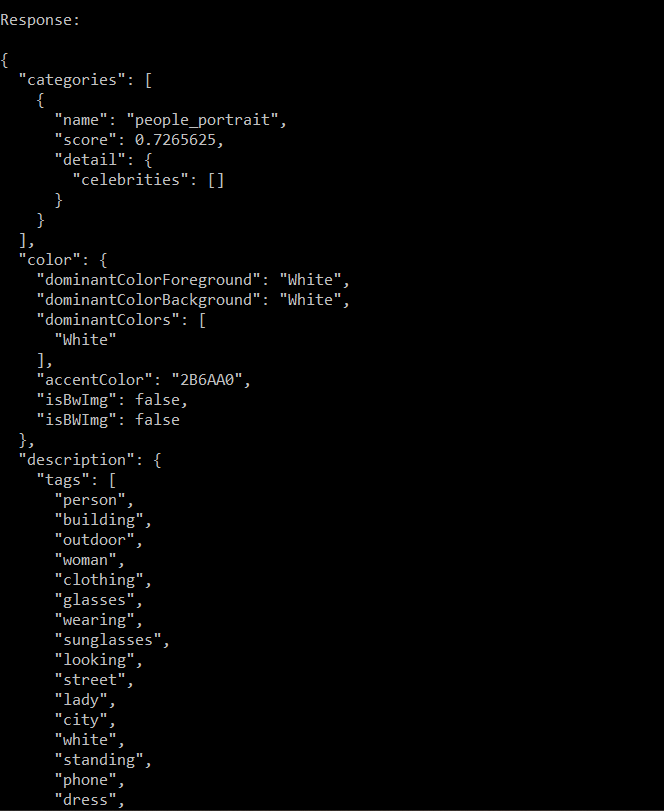
\includegraphics[scale=0.8]{JSONPICTURE.png}
    \caption{In deze figuur zie je het resultaat van de Microsoft foto-analyse API op een foto waarin een persoon voorkomt.}
    \label{fig:jsonfoto}
\end{figure}


De resultaten zijn opgedeeld in verschillende delen.\\ Als eerste wordt de foto aan een categorie toegekend; ind dit geval beslist de API dat de foto tot de \textbf{categorie} "people\_portrait" behoort. 

Daarna volgt een gedetailleerde beschrijving onder de vorm van \textbf{tags}. De eerste tags zoals 'person' en 'outdoor' zijn correct. Als we wat verder kijken in de lijst zien we enkele tags die niet bij de foto horen, zoals sunglasses, phone, en zelfs 'man'. 

Als laatste biedt de API nog een \textbf{conclusie-zin} aan die toont wat als hoofdelement op de foto herkend wordt. De zin 'a woman wearing glasses' is opvallend correct. 
De ander weergegeven info zoals formaat en dominante kleur zijn minder interessant binnen de scope van de GDPR.

\subsubsection{Stap 3: Resultaten gebruiken om PII-bevattende foto's te verwijderen.}
In deze stap is de applicatie verder ontwikkeld zodat hij niet langer toont welke informatie er in de foto's staat, maar aan de hand van deze informatie bepaalde foto's verwijdert. 

Dit gaat als volgt in z'n werk: Microsoft biedt \textbf{57 herkenbare categorieën} aan. Deze kunnen worden onderverdeeld in categoriën die mogelijk wijzen op aanwezigheid van persoonlijke info, en neutrale categorieën. Opgelet: dit is een eigen keuze voor elke onderneming die dit implementeert, veel categorieën zijn voor disucussie vatbaar. Bijvoorbeeld: alle categorieëen met 'Building'. Deze gebouwen kunnen huizen zijn, die dus verwijzen naar personen, of fabrieken die helemaal geen persoonlijke info bevatten. Op welke categorieën gefilterd wordt is dus een afweging die moet genomen worden. 
In dit onderzoek zijn volgende keuzes gemaakt: 

\textbf{Categorieën met mogelijk PII :}building\_, building\_arch, building\_brickwall, building\_church, building\_corner, building\_doorwindows, building\_pillar, building\_stair, building\_street, indoor\_, indoor\_churchwindow, indoor\_court, indoor\_doorwindows, indoor\_marketstore,
indoor\_room, 
,indoor\_venue \textbf{,people\_ ,people\_baby}
,people\_crowd
,people\_group
,people\_hand
,people\_many
,people\_portrait
,people\_show
,people\_tattoo
,people\_youngh
,people\_swimming
,text\_
,text\_mag
,text\_map
,text\_menu
,text\_sign
,outdoor\_pool ,trans\_bicycle

\textbf{Neutrale Categorieën:} abstract\_
,abstract\_net
,abstract\_nonphoto
,abstract\_rect
,abstract\_shape
,abstract\_texture
,animal\_
,animal\_bird
,animal\_cat
,animal\_dog
,animal\_horse
,animal\_panda
,dark\_
,drink\_
,drink\_can
,dark\_fire
,dark\_fireworks
,sky\_object
,food\_
,food\_bread
,food\_fastfood
,food\_grilled
,food\_pizza
,dark\_light
,others\_
,outdoor\_
,outdoor\_city
,outdoor\_field
,outdoor\_grass
,outdoor\_house
,outdoor\_mountain
,outdoor\_oceanbeach
,outdoor\_playground
,outdoor\_railway
,outdoor\_road
,outdoor\_sportsfield
,outdoor\_stonerock
,outdoor\_street
,outdoor\_water
,outdoor\_waterside
,plant\_
,plant\_branch
,plant\_flower
,plant\_leaves
,plant\_tree
,object\_screen
,object\_sculpture
,sky\_cloud
,sky\_sun

Dit is, binnen de applicatie, de \underline{eerste filter}. De input is een lijst met foto's.
Elke foto die door cognitive services wordt toegewezen aan een \textunderscore{categorie} van de eerste groep (categorie met mogelijk PII), wordt uit die lijst verwijderd. Hiermee zouden al alle foto's met mensen op moeten verwijderd zijn.

\subsubsection{stap 4: betrouwbaarheidstest}
Als test zijn 38 diverse foto's verzameld \textcite{Adobe2019}. Voornamelijk foto's van mensen in diverse situaties, met duidelijke/onduidelijke verlichting, achtergrond, enzoverder. 

Een voorbeeld van één van de foot's zie je in figuur 4.7.
\begin{figure}[h]
    
\includegraphics[scale=0.03]{fotosstest/1.jpg}
    \caption{In deze figuur zie je het resultaat van de Microsoft foto-analyse API op een foto waarin een persoon voorkomt..}
    \label{fig:fotopersoon}
\end{figure}
Daarnaast zijn ook foto's geselecteerd van huizen en andere gebouwen. De bedoeling is om te vergelijken hoeveel van deze foto's door de applicatie herkend worden als persoonlijke informatie bevattend, ten opzichte van wat de schrijvers van dit onderzoek van mening zijn. 


Na interpretatie van de foto's krijgen we volgende resultaten: 
\begin{itemize}
	\item Foto's herkend als PII door onderzoeker: 27/40
	\item Foto's herkend als PII door applicatie: 22/40
\end{itemize}
Deze resultaten vindt je terug in tabel 4.4. Als de menselijke interpretatie als correct wordt aanschouwd, maakt de API maar liefst 12 fouten.  

\begin{table}

\begin{tabularx}{\linewidth}{ |l|l|l|X| } 
	\hline
	Fotonummer & PII-onderzoeker & PII-applicatie & Fout  \\ [0.5ex]
	
	1 & Ja & Ja & \\
	2 & Ja & Ja & \\
	3 & Ja & Ja & \\
	4& Ja & Nee & \checkmark \\
	5& Ja & Nee & \checkmark \\
	6 & Ja & Ja & \\
	7 & Ja & Ja & \\
	8 & Ja & Nee & \checkmark \\
	9 & Ja & Ja & \\
	10 & Ja & Nee & \checkmark \\
	11 & Ja & Ja & \\
	12 & Ja & Ja & \\
	13 & Ja & Ja & \\
	14 & Nee & Nee & \\
	15 & Nee & Nee & \\
	16 & Ja & Nee & \checkmark \\
	17 & Ja & Ja & \checkmark  \\
	18 & Ja & Ja & \\
	19 & Ja & Nee & \checkmark \\
	20 & Ja & Ja & \\
	21 & Ja & Ja & \\
	22 & Ja & Ja & \\
	23 & Ja & Ja & \\
	24 & Ja & Ja & \\
	25 & Ja & Ja & \\
	26 & Ja & Ja & \\
	27 & Nee & Nee & \\
	28 & Ja & Nee & \checkmark \\
	29 & Nee & Nee & \\
	30 & Ja & Ja & \\
	31 & Nee & Ja & \checkmark \\
	32 & Nee & Nee & \\
	33 & Ja & Ja & \\
	34 & Nee & Ja & \checkmark \\
	35 & Nee & Nee & \\
	36 & Nee & Ja & \checkmark \\
	37 & Ja & Ja & \\
	38 & Ja & Nee & \checkmark \\
	\hline
	
\end{tabularx}
    \caption{Resultaat van de persoonlijke-informatie-herkenning in foto's. In de tweede kolom zie je of de foto door een mens is beoordeeld als persoonlijke informatie bevattend, in de derde kolom door de foto-analyse-API. In de vierde kolom staat een vinkje als kolom twee en drie verschillend zijn.}
\end{table}

\subsubsection{stap 5: Opkrikken betrouwbaarheidsniveau}
Het is duidelijk dat bij een aantal foto's de applicatie niet zegt: dit behoort tot een PII-categorie, terwijl dit wel zou moeten. Als dus enkel gefilterd wordt op categorie zijn de resultaten niet betrouwbaar.

Een volgende stap is om te kijken of dit kan verbeterd worden. Daarvoor worden de JSON resultaten van een foto die door de mens als PII herkend worden, maar niet door de applicatie, getoond in figuur 4.8. 

\begin{figure}[h]
	\centering
	\begin{subfigure}{0.45\textwidth}
		\centering
		
\includegraphics[width=.7\linewidth]{Fotosstest/2.jpg}
		\caption{Figuur met mensen op}
		\label{fig:qsdfqsdf}
	\end{subfigure}%
	\begin{subfigure}{0.45\textwidth}
		\centering
		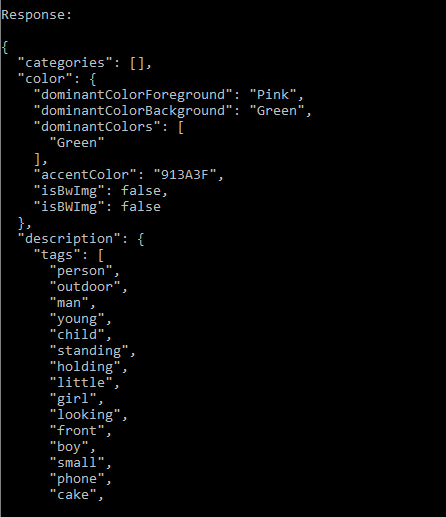
\includegraphics[width=.7\linewidth]{Fotosstest/2a.PNG}
		\caption{JSON resultaat na analyse foto a.}
		\label{fig:sub2}
	\end{subfigure}
	\caption{Deze foto (a) werd door de API niet toegewezen aan een categorie die PII kan bevatten. Dat zie je op foto b.}
	\label{fig:teqsdfqsdfst}
\end{figure}

Cognitive services is er voor deze foto niet in geslaagd om een categorie toe te kennen aan de foto. \textbf{Maar tussen de tags staat wel helemaal bovenaan: 'person'.} Dit doet vermoeden dat wanneer er bijkomend op tags gefilterd wordt, er beter betrouwbare resultaten kunnen geboekt worden. 

Volgende tags worden toegevoegd als filter in de applicatie: 'person', 'child', 'young', 'man', 'girl', 'boy', 'girl'.

Als nu een nieuwe betrouwbaardheidstest wordt gedaan krijgen we volgende resultaten: 
\begin{itemize}
	\item Foto's herkend als PII door onderzoeker: 27/40
	\item Foto's herkend als PII door applicatie: 31/40
\end{itemize}

Er worden iets meer foto's als PII aanzien, maar het belangrijkste voor deze applicatie is dat er geen foto's meer waarin mensen herkend worden, niet gefilterd worden. 
Dat er iets te veel foto's herkend zijn kan zorgen voor een onnodig verlies van data, maar is veiliger dan wanneer er net ies te weinig foto's zouden herkend zijn. Elke onderneming kan door tags en categorieën te kiezen zelf bepalen hoe 'streng' de filter is. 


\subsection{Resultaat console-applicaties}
Er kan geconcludeerd worden dat de textanalyse-API van Microsoft nog niet klaar is om alle persoonlijke data uit tekst te herkennen, zeker niet als deze tekst in verschillende talen voorkomt.
Waar de herkenning wel plaatsvindt is het filteren van persoonlijke data wel succesvol, dus de ontwikkelde applicatie kan dienen als een eerste tijdelijke stap bij een aanvraag tot verwijderen van persoonlijke data. (Bijvoorbeeld tot één van de werknemers tijd heeft om manueel gaat controleren op persoonlijke data.) 
Zeker als door middel van Reguliere Expressies, vast voorkomende vormen van data (zoals tags), worden gefilterd. 

Waar de text-analyse nog te kort schiet lijkt de foto-analyse wel al klaar voor gebruik. Er is op een geslaagde manier een applicatie ontwikkeld die persoonlijk informatie bevattende foto's herkent. 



https://gdpr-info.eu/recitals/ bijlage
Recital 26
1The principles of data protection should apply to any information concerning an identified or identifiable natural person. 2Personal data which have undergone pseudonymisation, which could be attributed to a natural person by the use of additional information should be considered to be information on an identifiable natural person. 3To determine whether a natural person is identifiable, account should be taken of all the means reasonably likely to be used, such as singling out, either by the controller or by another person to identify the natural person directly or indirectly. 4To ascertain whether means are reasonably likely to be used to identify the natural person, account should be taken of all objective factors, such as the costs of and the amount of time required for identification, taking into consideration the available technology at the time of the processing and technological developments. 5The principles of data protection should therefore not apply to anonymous information, namely information which does not relate to an identified or identifiable natural person or to personal data rendered anonymous in such a manner that the data subject is not or no longer identifiable. 6This Regulation does not therefore concern the processing of such anonymous information, including for statistical or research purposes.

Grond 75
EU-AVG
(75) Het qua waarschijnlijkheid en ernst uiteenlopende risico voor de rechten en vrijheden van natuurlijke personenkan voortvloeien uit persoonsgegevensverwerking die kan resulteren in ernstige lichamelijke, materiële of immateriële schade, met name: waar de verwerking kan leiden tot discriminatie, identiteitsdiefstal of -fraude, financiële verliezen, reputatieschade, verlies van vertrouwelijkheid van door het beroepsgeheim beschermde persoonsgegevens, ongeoorloofde ongedaanmaking van pseudonimisering, of enig ander aanzienlijk economisch of maatschappelijk nadeel; wanneer de betrokkenen hun rechten en vrijheden niet kunnen uitoefenen of worden verhinderd controle over hun persoonsgegevens uit te oefenen; wanneer persoonsgegevens worden verwerkt waaruit ras of etnische afkomst, politieke opvattingen, religie of levensbeschouwelijke overtuigingen, of vakbondslidmaatschap blijkt, en bij de verwerking van genetische gegevens of gegevens over gezondheid of seksueel gedrag of strafrechtelijke veroordelingen en strafbare feiten of daarmee verband houdende veiligheidsmaatregelen; wanneer persoonlijke aspecten worden geëvalueerd, om met name beroepsprestaties, economische situatie, gezondheid, persoonlijke voorkeuren of interesses, betrouwbaarheid of gedrag, locatie of verplaatsingen te analyseren of te voorspellen, teneinde persoonlijke profielen op te stellen of te gebruiken; wanneer persoonsgegevens van kwetsbare natuurlijke personen, met name van kinderen, worden verwerkt; of wanneer de verwerking een grote hoeveelheid persoonsgegevens betreft en gevolgen heeft voor een groot aantal betrokkenen.